\documentclass[a4paper, article]{article}

\usepackage{fontspec}
\usepackage[14pt]{extsizes}
\setmainfont{Times New Roman}

\usepackage[english, russian]{babel}

\usepackage[left=2cm, top=2cm, right=1cm, bottom=2cm]{geometry}
\usepackage[onehalfspacing]{setspace}

\usepackage{indentfirst}

\usepackage{titlesec}
\titleformat{\section}
{\centering\normalfont\bfseries}{\thesection. }{0em}{}
\titleformat{\subsection}
{\centering\normalfont\bfseries}{\thesubsection. }{0em}{}

\usepackage{xltabular}

\usepackage{graphicx}
\usepackage{float}
\usepackage{wrapfig}
\graphicspath{{images/}}
\usepackage[labelsep=period]{caption}
\makeatletter
\renewcommand{\fnum@figure}{Рисунок \thefigure}
\makeatother

\begin{document}
    \begin{titlepage}
        \begin{center}
            {\bf Министерство науки и высшего образования Российской Федерации \\
            Федеральное государственное автономное образовательное учреждение \\
            высшего образования \\
            <<КАЗАНСКИЙ (ПРИВОЛЖСКИЙ) ФЕДЕРАЛЬНЫЙ УНИВЕРСИТЕТ>>}

            \vspace{2em}

            {ИНСТИТУТ ВЫЧИСЛИТЕЛЬНОЙ МАТЕМАТИКИ И \\
            ИНФОРМАЦИОННЫХ ТЕХНОЛОГИЙ}

            \vspace{2em}

            {КАФЕДРА АНАЛИЗА ДАННЫХ И \\
            ТЕХНОЛОГИЙ ПРОГРАММИРОВАНИЯ}

            \vspace{6em}

            ОТЧЁТ \\
            {\bf ПО ЛАБОРАТОРНОЙ РАБОТЕ \\
            <<МОДЕЛИРОВАНИЕ ДИПЛОМНОЙ РАБОТЫ>>}
        \end{center}

        \vfill

        \begin{xltabular}{\textwidth} {
                >{\hsize=0.5\hsize} X
                >{\hsize=0.5\hsize} X }
            \bf{Работа выполнена:} & \\
            Студент 4 курса группы 09-951 & \hspace{2cm}Колесников Д.А.\\
            & \\
            \bf{Работа проверена:} & \\
            Старший преподаватель & \hspace{2cm}Жажнева И.В. \\
        \end{xltabular}

        \vspace{2em}

        \begin{center}
            Казань — 2023
        \end{center}
    \end{titlepage}

    \pagebreak

    \setcounter{page}{2}

    \tableofcontents

    \pagebreak

    \section{Система из ВКР}

    \subsection{Обзор}

    Моя тема вкр -- <<Система записи в медицинское учреждение>>. Примерные функции, которые должны быть в приложении:

    \vspace{-1em}
    \begin{itemize}
        \setlength\itemsep{0em}

        \item Врач указывает время своего приёма
        \item Регистратура записывает пациента к врачу
        \item В случае невозможности встречи регистратор меняет запись
        \item Регистратор может менять инфорамцию о человеке
        \item Врач может менять информацию о пациенте и его болезни
        \item Генерация отчётов
    \end{itemize}

    \subsection{Рамки модели}

    В рамках этой работы мы смоделируем только момент, касающийся записи поциента регистратором. Можно написать алгоритм этой задачи:

    \vspace{-1em}
    \begin{enumerate}
        \setlength\itemsep{0em}

        \item Пациент приходит в поликлинику
        \item Идёт в зал ожидания
        \item Подходит в свободное окно регистратуры
        \item Регистратор его записывает
        \item Пациент освобождает окно регистратуры
        \item Уходит из поликлиники
    \end{enumerate}

    Дальше процесс регистратуры не касается и его моделирование -- отдельная задача. Значит можем выделить сущности: поликлиника, пациент, регистратор. Далее займёмся реализацией.

    \pagebreak

    \section{AnyLogic}

    \subsection{Обзор}

    AnyLogic - система имитационного моделирования. Создана на Java и поддерживает графический язык моделирования, который переводится в Java. Включает в себя много библиотек для разных ситуаций.

    \subsection{Применение}

    Нужно сделать пространство, в котором будут находиться объекты. То есть создать <<поликлинику>>. С помощью встроенных в AnyLogic средств сделаем это. Результат на Рисунке~\ref{fig:page2dPlan}.

    \begin{figure}[h]
        \centering
        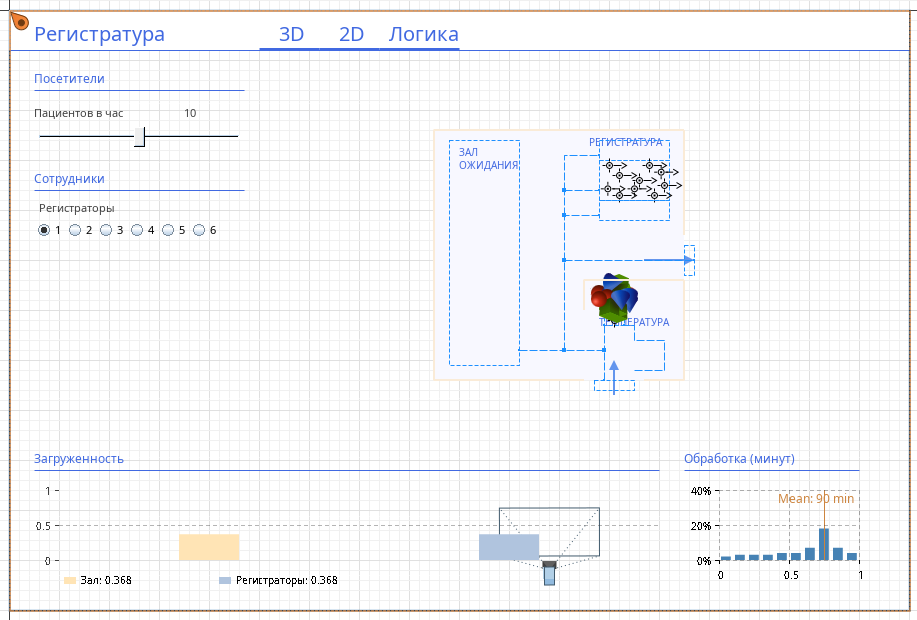
\includegraphics[width=0.7\linewidth]{page2dPlan.png}
        \caption{\centering Визуальная модель}
        \label{fig:page2dPlan}
    \end{figure}

    Здесь оранжевое -- стены, синее -- пол. Яркие синие полосы -- пути, по которм могут ходить пациенты. Стрелками указаны вход в выход. Много точек сверху справа - регистраторы. 3D-фигура -- стойка для проверки темпаратуры. Справа выставим параметры -- интенсивность пациентов и количество регистраторов. Снизу будет показываться загруженность элементов поликлиники.

    Для этой модели нужно сделать логику. Она представлена на Рисунке~\ref{fig:pageLogicSource}.

    \begin{figure}[h]
        \centering
        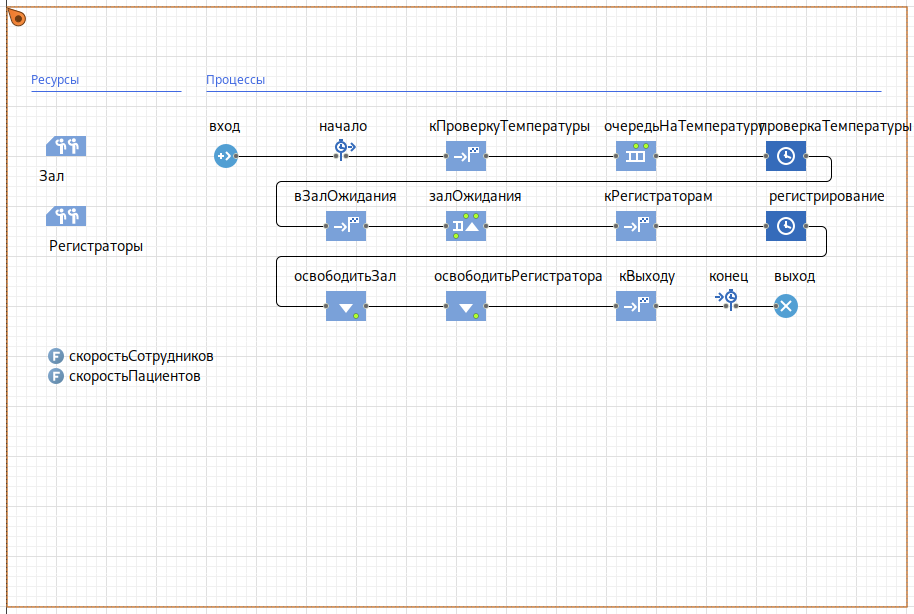
\includegraphics[width=0.7\linewidth]{pageLogicSource.png}
        \caption{\centering Написанная логика модели}
        \label{fig:pageLogicSource}
    \end{figure}

    Здесь выражены 3 этапа: подготовка, регистрирование, завершение. Они визуально разделены на 3 уровня. В первой строке пациент приходит в поликлинику и проверяет температуру. Во второй он ждёт своей очереди в регистратуру в зале и, когда наступает момент, идёт регистрироваться. В третьей строке пациент всё сделал и ему осталось уйти -- освободить регистратуру и помещение. На этом моделирование отдельного пациента заканчивается.

    \pagebreak

    \section{Сделанная модель}

    \subsection{3D}

    Запустим модель в AnyLogic. По умолчанию у меня открывается 3D-модель, представленная на Рисунке~\ref{fig:page3d}. Здесь видны поставленные стены, пол, люди, стол. 3D модели лежат в отдельной папке в папке проекта. Они взяты со стороннего проекта. Человечки здесь перемещаются, можно в реальном времени в 3D видеть процесс.

    \begin{figure}[h]
        \centering
        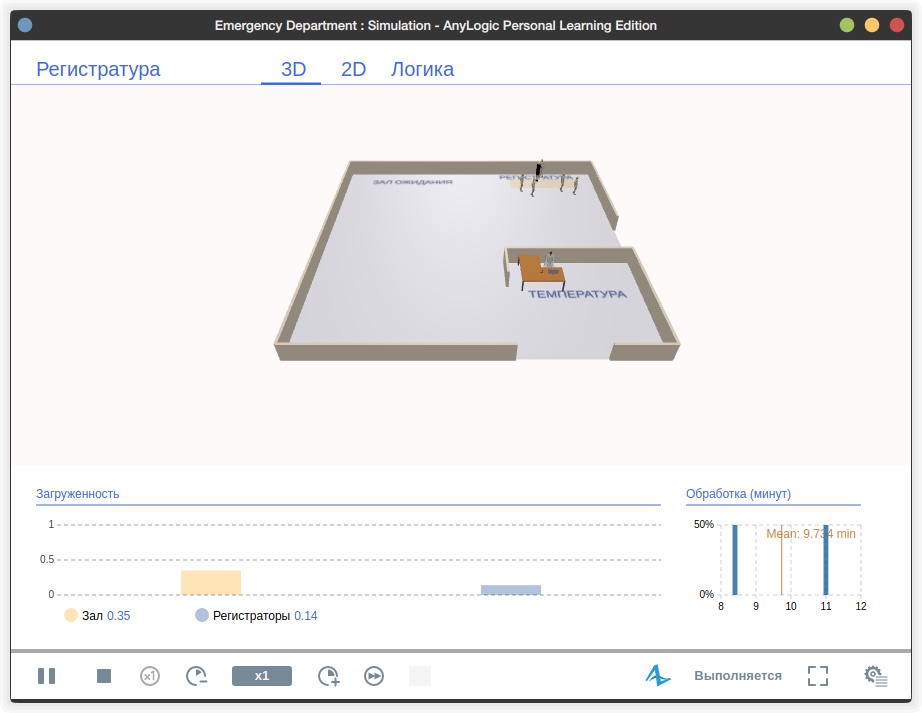
\includegraphics[width=0.7\linewidth]{page3d.png}
        \caption{\centering 3D-режим модели}
        \label{fig:page3d}
    \end{figure}

    \pagebreak

    \subsection{2D}

    Вторая вкладка -- модель в 2D. Здесь уже можно настраивать параметры. Так, если поставить 1 человека в час, то поликлиника будет простаивать, а если 15 -- будет забита. В остальном этот режим не отличается от 3D. Те же графики, та же поликлиника.

    \begin{figure}[h]
        \centering
        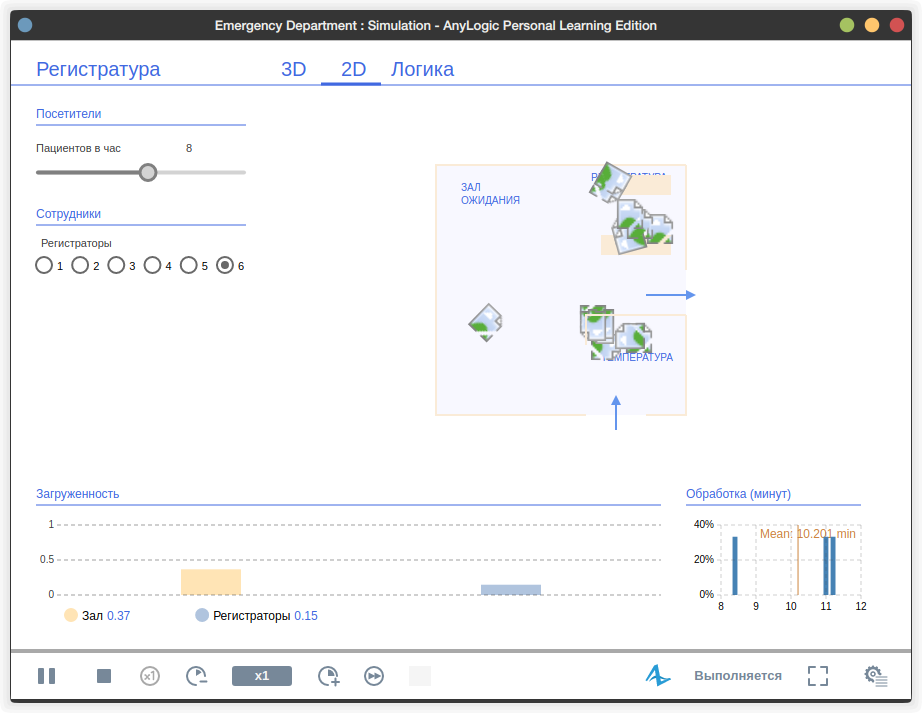
\includegraphics[width=0.7\linewidth]{page2d.png}
        \caption{\centering 2D-режим модели}
        \label{fig:page2d}
    \end{figure}

    \pagebreak

    \subsection{Логика}

    Последний режим -- режим просмотра работы логики модели. Мы её создали, но не могли отслеживать состояние в реальном времени. Теперь можем. У каждого элемента написано сколько человек через него прошло. Так, например, зашли в поликлинику 25 человек, а вышло 24. При этом загруженность регистраторов - 27\%. Значит один человек находится в поликлинике и он сейчас у регистратора.

    \begin{figure}[h]
        \centering
        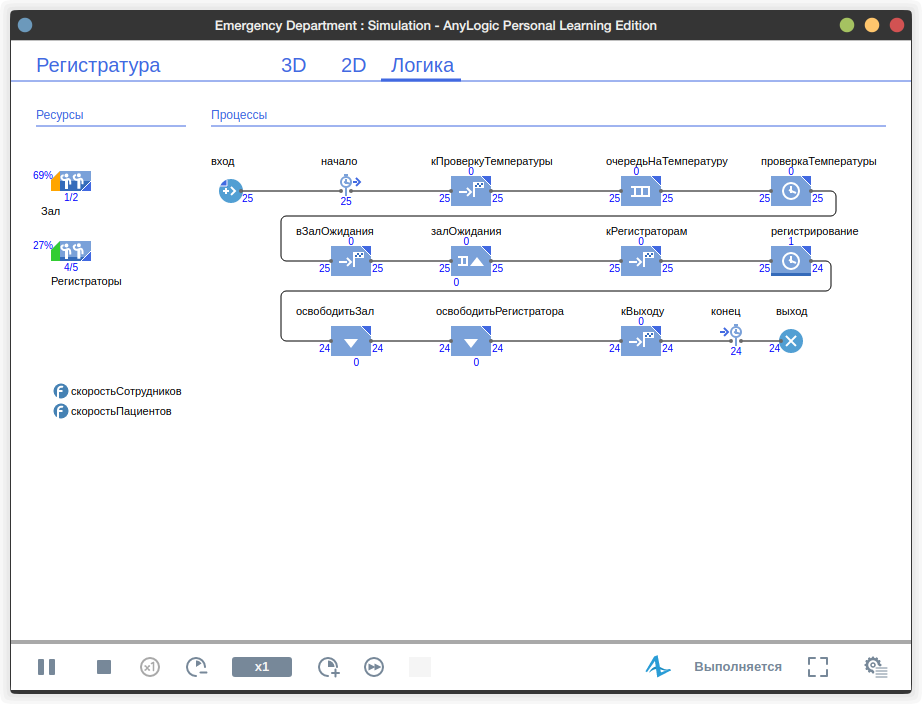
\includegraphics[width=0.7\linewidth]{pageLogic.png}
        \caption{\centering Логика в процессе выполнения}
        \label{fig:pageLogic}
    \end{figure}

    \pagebreak

    \section*{Заключение}
    \addcontentsline{toc}{section}{Заключение}

    В ходе работы создана модель, описывающая один из процессов для моего диплома. Модель создана с помощью инструмента имитационного моделирования -- AnyLogic. На основе этой системы можно делать определённые выводы о том, к какой производительности должна стремиться система. Либо, например, сколько для корректной работы нужно поставить регистраторов.

\end{document}
